\documentclass[12pt]{article}
\usepackage[left=1cm, right=1cm, top=2cm,bottom=1.5cm]{geometry} 

\usepackage[parfill]{parskip}
\usepackage[utf8]{inputenc}
\usepackage[T2A]{fontenc}
\usepackage[russian]{babel}
\usepackage{enumitem}
\usepackage[normalem]{ulem}
\usepackage{amsfonts, amsmath, amsthm, amssymb, mathtools}
\usepackage{tikz}
\usepackage{tabularx}
\usepackage{hhline}

\usepackage{accents}
\usepackage{fancyhdr}
\pagestyle{fancy}
\renewcommand{\headrulewidth}{1.5pt}
\renewcommand{\footrulewidth}{1pt}

\usepackage{graphicx}
\usepackage[figurename=Рис.]{caption}
\usepackage{subcaption}
\usepackage{float}

%%Наименование папки откуда забирать изображения
\graphicspath{ {./images/} }

%%Изменение формата для ввода доказательства
\renewcommand{\proofname}{$\square$  \nopunct}
\renewcommand\qedsymbol{$\blacksquare$}

%%Изменение отступа на таблицах
\addto\captionsrussian{%
	\renewcommand{\proofname}{$\square$ \nopunct}%
}
%% Римские цифры
\newcommand{\RN}[1]{%
	\textup{\uppercase\expandafter{\romannumeral#1}}%
}

%% Для удобства записи
\newcommand{\MR}{\mathbb{R}}
\newcommand{\MQ}{\mathbb{Q}}
\newcommand{\MC}{\mathbb{C}}
\newcommand{\MI}{\mathrm{I}}
\newcommand{\MJ}{\mathrm{J}}
\newcommand{\MH}{\mathrm{H}}
\newcommand{\MT}{\mathrm{T}}
\newcommand{\MU}{\mathcal{U}}
\newcommand{\MV}{\mathcal{V}}
\newcommand{\VN}{\varnothing}
\newcommand{\VE}{\varepsilon}

\theoremstyle{definition}
\newtheorem{defn}{Опр:}
\newtheorem{rem}{Rm:}
\newtheorem{prop}{Утв.}
\newtheorem{exrc}{Упр.}
\newtheorem{lemma}{Лемма}
\newtheorem{theorem}{Теорема}
\newtheorem{corollary}{Следствие}

\newenvironment{cusdefn}[1]
{\renewcommand\thedefn{#1}\defn}
{\enddefn}

\DeclareRobustCommand{\divby}{%
	\mathrel{\text{\vbox{\baselineskip.65ex\lineskiplimit0pt\hbox{.}\hbox{.}\hbox{.}}}}%
}
%Короткий минус
\DeclareMathSymbol{\SMN}{\mathbin}{AMSa}{"39}
%Длинная шапка
\newcommand{\overbar}[1]{\mkern 1.5mu\overline{\mkern-1.5mu#1\mkern-1.5mu}\mkern 1.5mu}
%Функция знака
\DeclareMathOperator{\sgn}{sgn}

%Обозначение константы
\DeclareMathOperator{\const}{\text{const}}

%Интеграл в большом формате
\DeclareMathOperator{\dint}{\displaystyle\int}

\newcommand{\smallerrel}[1]{\mathrel{\mathpalette\smallerrelaux{#1}}}
\newcommand{\smallerrelaux}[2]{\raisebox{.1ex}{\scalebox{.75}{$#1#2$}}}

\newcommand{\smallin}{\smallerrel{\in}}
\newcommand{\smallnotin}{\smallerrel{\notin}}

\newcommand*{\medcap}{\mathbin{\scalebox{1.25}{\ensuremath{\cap}}}}%
\newcommand*{\medcup}{\mathbin{\scalebox{1.25}{\ensuremath{\cup}}}}%

%Скалярное произведение
\DeclarePairedDelimiterX{\inner}[2]{\langle}{\rangle}{#1, #2}

%Подпись символов снизу
\newcommand{\ubar}[1]{\underaccent{\bar}{#1}}

\newcommand*\circled[1]{\tikz[baseline=(char.base)]{
		\node[shape=circle,draw,inner sep=2pt] (char) {#1};}}


\begin{document}
\lhead{Наглядная геометрия и топология}
\chead{Ошемков А.А.}
\rhead{Лекция - 1}
\section*{Введение по курсу}
Данный курс - введение в различные разделы геометрии и топологии.

Пример задач, обсуждаемых на курсе: сжимание замкнутой кривой на сфере - можно сжать в точку. На торе, например, есть кривые, которые не получится сжать в точку без разрывов не деформируя непрерывности. В некотором смысле стягивание в точку это харакрестический показать: если на двумерной поверхности любая замкнутая кривая стягивается в точку, то это сфера.
\begin{figure}[H]
	\centering
	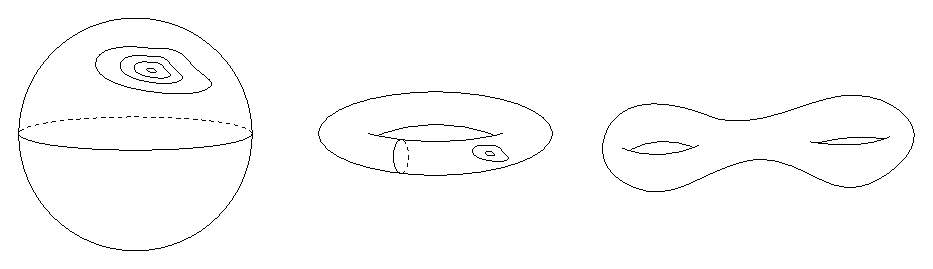
\includegraphics[width=0.85\textwidth]{1_1.eps}
	\caption{Примеры изучаемых объектов.}
	\label{1_1}
\end{figure}

\section*{Графы}

Впервые идея использовать графы пришла Эйлеру при решении задачи о Кёнигсбергских мостах.
\begin{figure}[H]
	\centering
	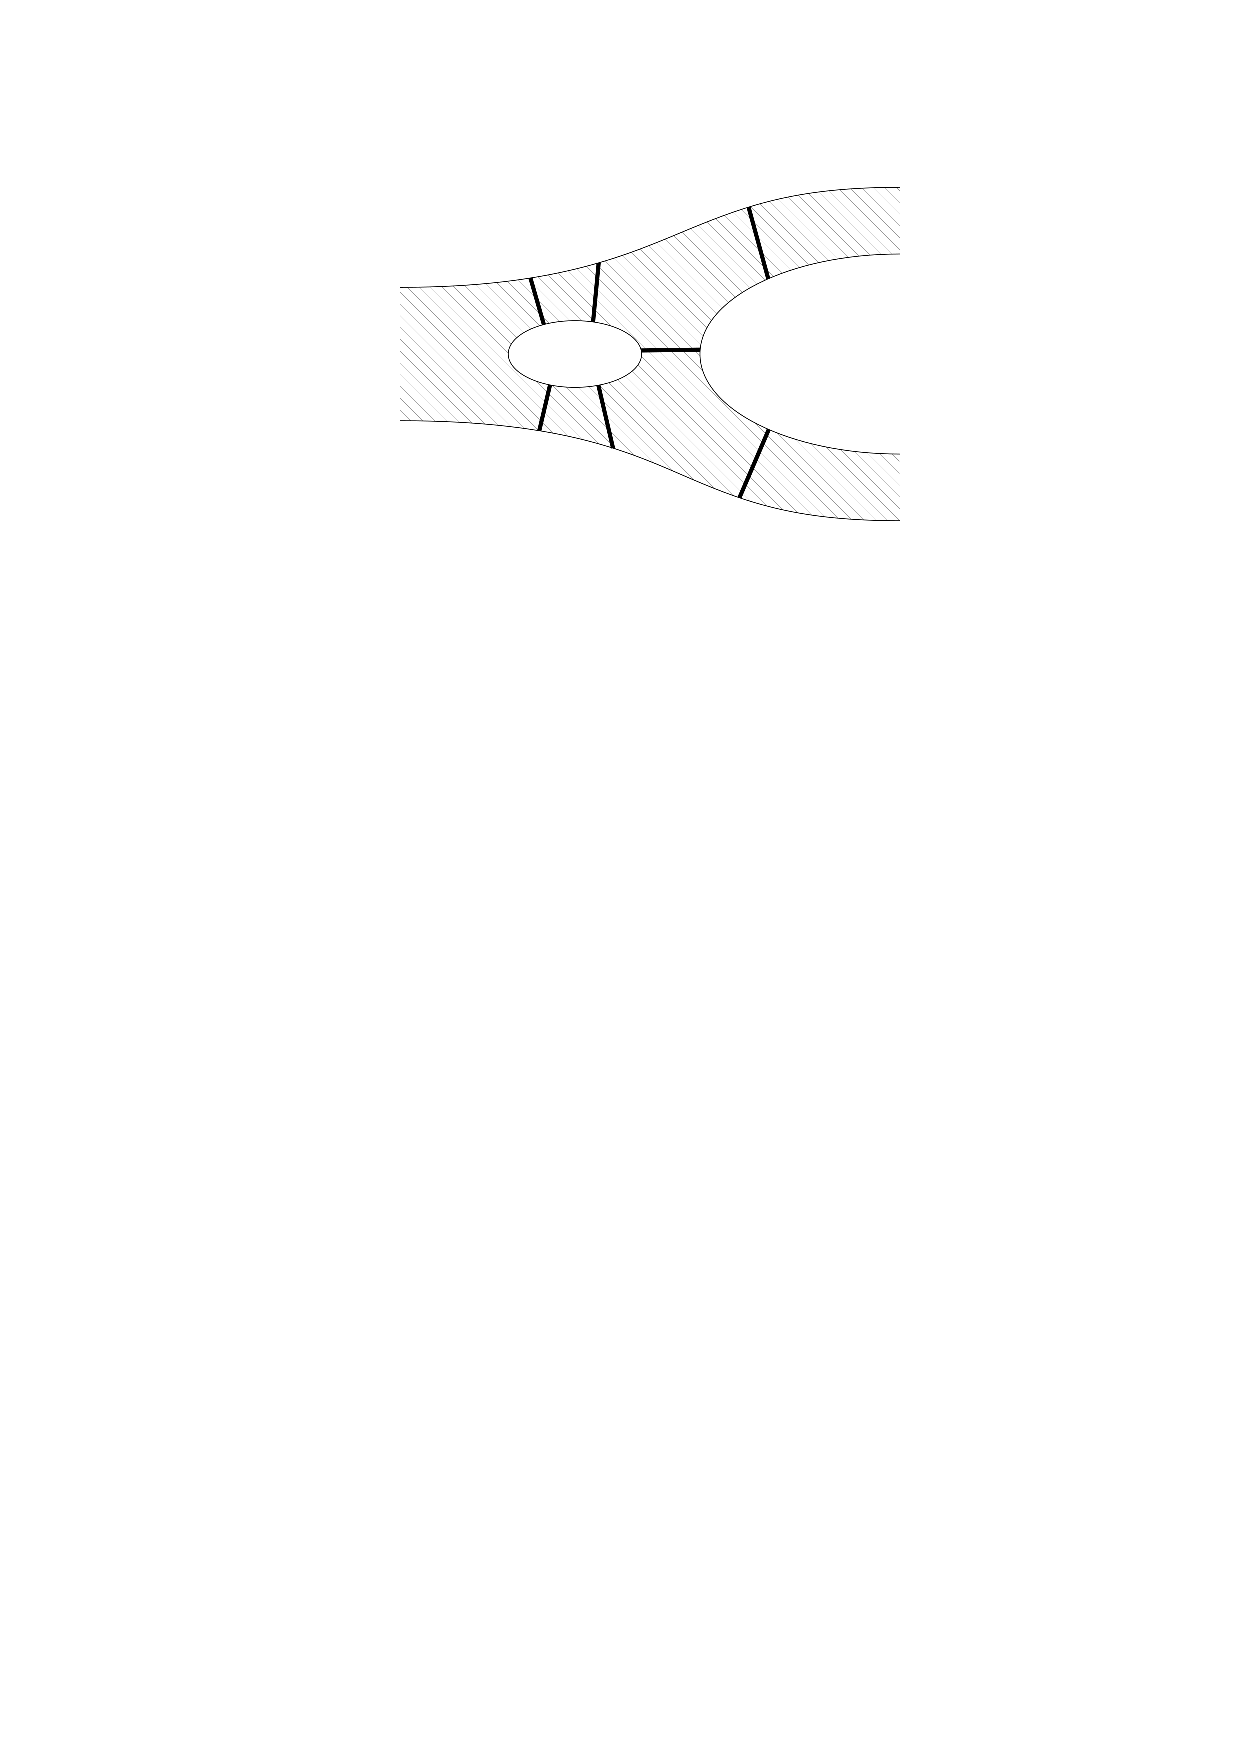
\includegraphics[width=0.3\textwidth]{1_2.png}
	\caption{Задача о 7 Кёнигсбергских мостах.}
	\label{1_2}
\end{figure}
Можно ли прогуляться по всем 7-ми мостам, начав с какой-то точки, пройдя по каждому мосту только один раз и вернуться в ту же точку.

\begin{figure}[H]
	\centering
	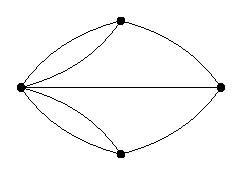
\includegraphics[width=0.25\textwidth]{1_3.eps}
	\caption{Граф Кёнигсбергсих мостов.}
	\label{1_3}
\end{figure}
Перформулируя задачу в граф: получим 4 вершины и 7 ребер. Можем ли, стартуя в какой-то вершине, пройти по всем ребрам графа так, чтобы по каждому ребру пройтись один раз и вернуться в исходную точку? Ответ - нет. Чтобы это было возможно сделать, все вершины должны иметь четную степень (количество ребер подходящих к вершинам).

\subsection*{Комбинаторное описание графов}
Чтобы описать граф, не обязательно рисовать картинку. Рассмотрим множества:

\begin{defn}
	\uwave{Граф} это набор множеств $(V,E)$, где $V$ - конечное непустое множество, элементы которого будем называть \uwave{вершинами} и $E$ - набор неупорядоченных пар вершин, элементы которого будем называть \uwave{ребрами}.
\end{defn}

\textbf{Пример}: $V = \{1,2,3,4\}; \, E: (1,2),\, (1,2),\,(2,3),\,(1,3)\,(1,4),\,(1,4),\,(3,4), \, (3,3)$.

\begin{figure}[H]
	\centering
	\includegraphics[width=0.35\textwidth]{1_4.eps}
	\caption{Комбинаторное описание графа.}
	\label{1_4}
\end{figure}

\begin{defn}
	Если какое-то ребро встречается $k$ раз, то говорят, что это \uwave{ребро кратности $k$}.
\end{defn}

\begin{defn}
	Если ребро состоит из одинаковых элементов, то такое ребро называется \uwave{петлей}.
\end{defn}

\textbf{Пример}: $(3,3)$ - это петля.

\begin{defn}
	\uwave{Степень вершины} - чиcло раз, сколько встречается эта вершина в наборе из ребер.
\end{defn}

\textbf{Пример}: степень вершины $2$ равна $3$, степень вершины $3$ равна $5$.

\subsection*{Геометрическое описание графов}
Почему это может интересовать? Например, есть желание положить граф на плоскость, возможно ли это?\\
\textbf{\uline{Напоминание}}: $f$ \uwave{непрерывна в точке} $x_0$, если 
$$\forall \VE > 0, \exists \, \delta > 0 \colon |x - x_0| < \delta \Rightarrow |f(x) - f(x_0)| < \VE$$

Немного другими словами, функция $f$ \uwave{непрерывна в точке} $x_0$, если для любой окрестности $W$ точки $y_0 = f(x_0)$ существует окрестность $U$ точки $x_0$, такая что $f(U) \subset W$.

В этой переформулировке нет упоминания о числах. В этом случае, при отображении каких-то пространств, в которых есть окрестности точек, мы получим определение непрерывности этого отображения.

\begin{figure}[H]
	\centering
	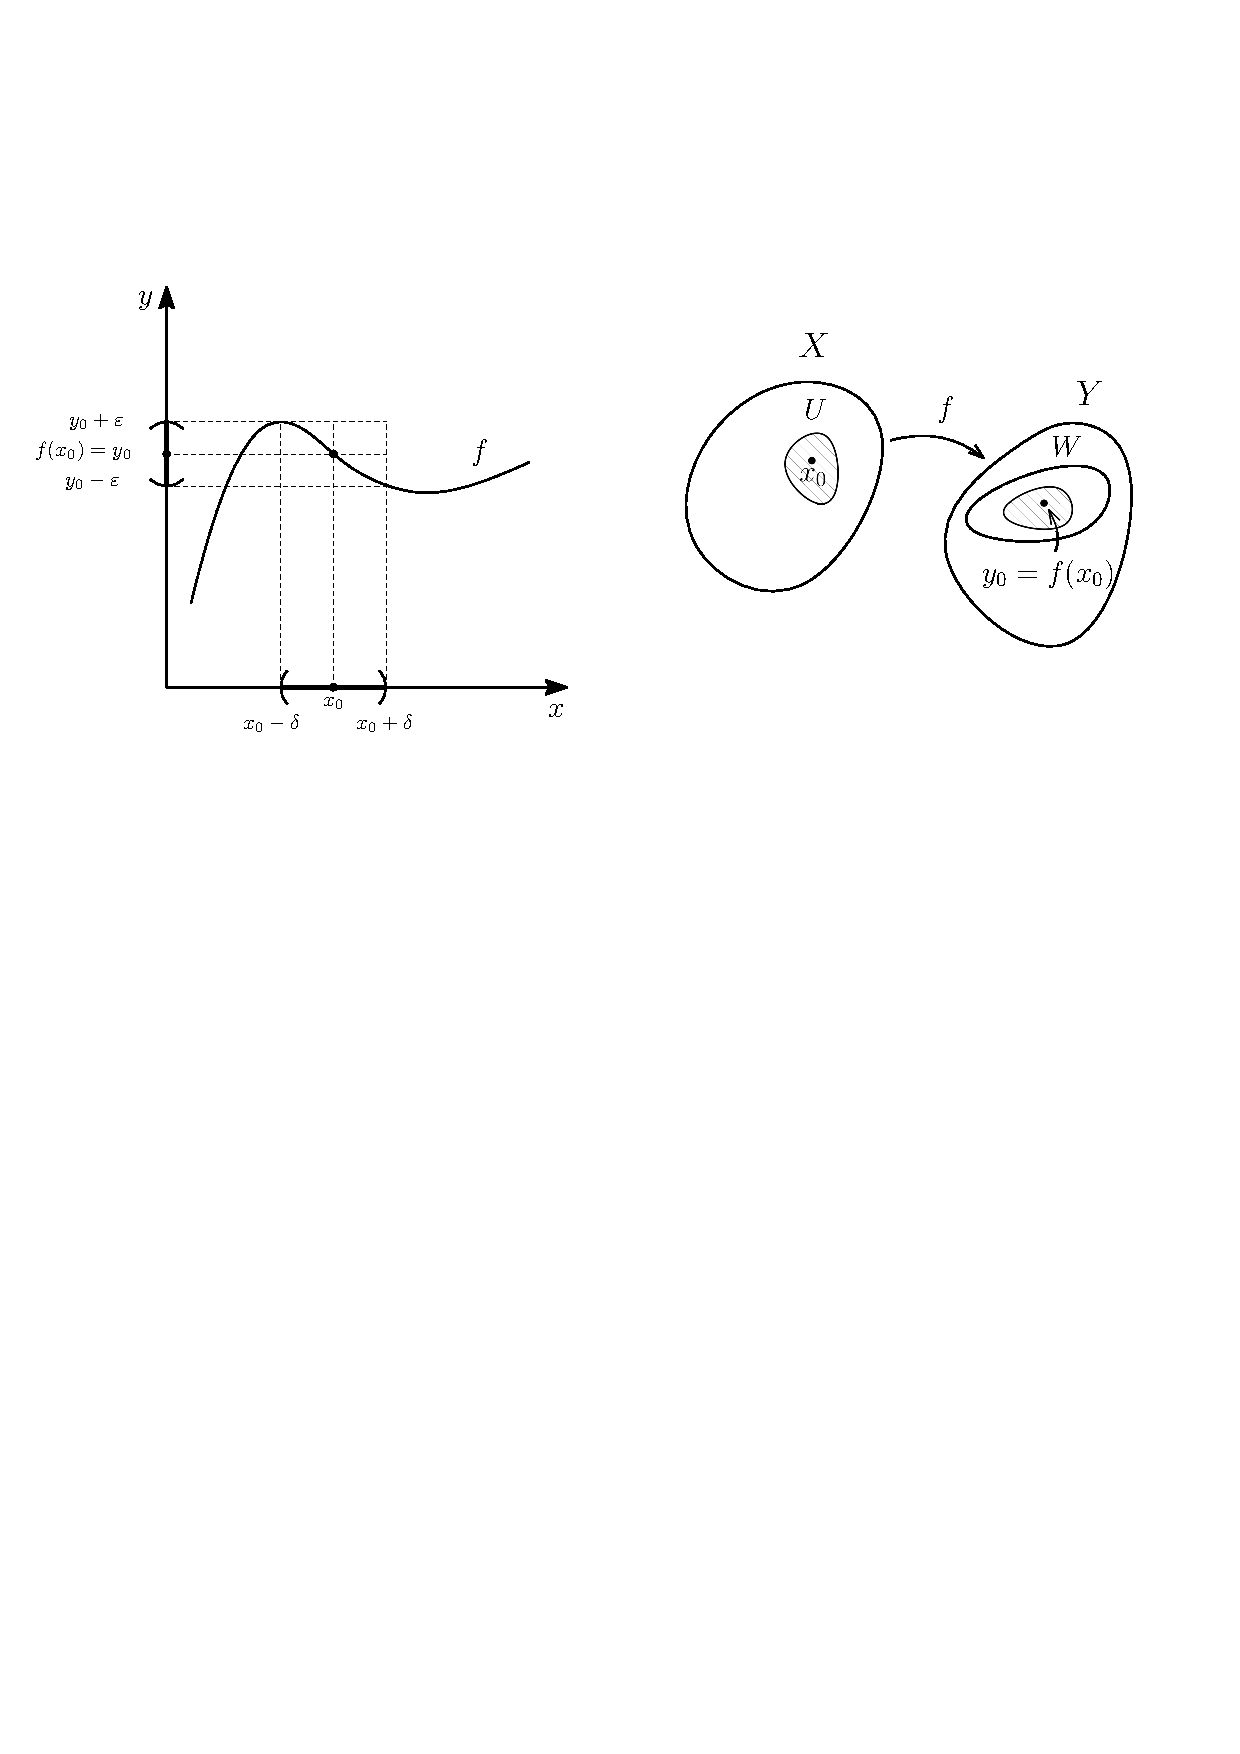
\includegraphics[width=0.8\textwidth]{1_5.png}
	\caption{Непрерывность функции в точке $x_0$.}
	\label{1_5}
\end{figure}

На числовой прямой под отрезком понимается множество точек $\{\,x \mid  a\leq x \leq b \,\}$. Когда будем говорить про отрезки - нам будет неважно, какие у него концы и если будем рассматривать несколько отрезков, можем представлять каждый отрезок на своей прямой.

\begin{defn}
	\uwave{Граф} это тройка объектов $(V,E,\partial)$:
	\begin{enumerate}[label ={(\arabic*)}]
		\item $V$ - конечное непустое множество, элементы которого будем называть \uwave{вершинами};
		\item $E$ - конечный набор отрезков, которые будем называть \uwave{ребрами};
		\item $\partial \colon \text{(множество концов отрезков из } E ) \to V$, которое будем называть \uwave{приклеиванием отрезков} к вершинам;
	\end{enumerate}
	Граф имеет два типа точек: 
	\begin{enumerate}[label ={(\arabic*)}]
		\item Вершины (элементы $V$);
		\item Внутренние точки ребер (отрезков из $E$);
	\end{enumerate}
	При этом:
	\begin{enumerate}[label ={(\arabic*)}]
		\item окрестность внутренней точки ребра - как в обычном отрезке (интервал);
		\item окрестность вершины $v$ - есть объединение окрестностей всех точек из $\partial^{\SMN1}(v)$ и самой вершины; 
	\end{enumerate}
\end{defn}

\begin{figure}[H]
	\centering
	\includegraphics[width=0.85\textwidth]{1_6.eps}
	\caption{Граф.}
	\label{1_6}
\end{figure}

\begin{rem}
	Если $\partial^{\SMN1}(v) = \VN$, то окрестность самой вершины будет состоять только из неё самой.
\end{rem}
\begin{rem}
	При рассмотрении отрезка $[a,b]$, окрестностью точки $a$ будет полуинтервал $[a, a+ \VE)$.
\end{rem}

\begin{figure}[H]
	\centering
	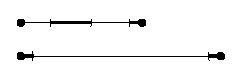
\includegraphics[width=0.3\textwidth]{1_7.eps}
	\caption{Окрестности точек в графе.}
	\label{1_7}
\end{figure}
Рассмотрим пространство $\MR^2$. На нем, расстояние между точками определяется как обычное Евклидово расстояние: 
$$
	\rho(A,B) = \sqrt{(a_1 - b_1)^2 + (a_2 - b_2)^2}
$$ 
\begin{figure}[H]
	\centering
	\includegraphics[width=0.3\textwidth]{1_8.png}
	\caption{Замкнутый шар в $\MR^2$.}
	\label{1_8}
\end{figure}
Тогда в качестве окрестности точки $P$ будем рассматривать шар.
\begin{defn}
	Множество точек  $B_{P,\VE} = \{\,x \in \MR^2 \mid \rho(P,x) < \VE \,\}$ называется \uwave{открытым шаром} с центром в точке $P$ и радиуса $\VE$.
\end{defn}
\begin{defn}
	Множество точек  $\overline{B}_{P,\VE} = \{\,x \in \MR^2 \mid \rho(P,x) \leq \VE \,\}$ называется \uwave{замкнутым шаром} с центром в точке $P$ и радиуса $\VE$.
\end{defn}
\begin{rem}
	На прямой открытый шар называют \uwave{интервалом}.
\end{rem}

\begin{defn}
	Пусть в пространствах $X$ и $Y$ заданы окрестности точек, причем для любой точки пересечение двух её окрестностей тоже является её окрестностью. Тогда  отображение $f\colon X \to Y$ \uwave{непрерывно в точке} $x_0 \in X$, если $\forall$ окрестности $W$ точки $y_0 = f(x_0), \, \exists$ окрестность $U$ точки $x_0$, такая что $f(U) \subset W$.
\end{defn}

\begin{defn}
	Отображение $f \colon X \to Y$ называется \uwave{непрерывным}, если оно непрерывно в каждой точке.
\end{defn}

\begin{defn}
	Подмножество $A\subset X$ (в котором заданы окрестности точек) называется \uwave{открытым}, если вместе с каждой точкой $a \in A$ оно содержит некоторую её окрестность. То есть:
	$$
	\forall a \in A, \exists \, \MU(a) \subset X \colon \MU(a) \subset A
	$$
\end{defn}

\begin{defn}
	Подмножество $A\subset X$ (в котором заданы окрестности точек) называется \uwave{замкнутым}, если его дополнение $X \setminus A$ - открыто (в $X$). То есть:
	$$
		\forall b \notin A, \exists \, \MU(b) \subset X \colon \MU(b) \cap A = \VN
	$$
\end{defn}

\begin{figure}[H]
	\centering
	\includegraphics[width=0.55\textwidth]{1_9.eps}
	\caption{Открытые ($A$) и замкнутые ($B$) подмножества $X$.}
	\label{1_9}
\end{figure}
\begin{rem}
	Открытое или замкнутое - зависит от того, в каком пространстве мы его рассматриваем.
\end{rem}

\textbf{Пример}: Пусть $X = \MR,\, A = [a,b]$ - не является открытым в $X$, но является замкнутым в $X$. Можно взять окрестность точки $b$ и целиком она не попадет в $A$;
\begin{figure}[H]
	\centering
	\includegraphics[width=0.35\textwidth]{1_10.eps}
	\caption{$A = [a,b]$ не является открытым подмножеством $X = \MR$.}
	\label{1_10}
\end{figure}
\textbf{Пример}: Пусть $X = [a,b],\, A = [a,b]$ - является открытым в $X$. Можно взять окрестность точки $b$ и целиком она попадет в $A$;
\begin{figure}[H]
	\centering
	\includegraphics[width=0.35\textwidth]{1_11.eps}
	\caption{$A = [a,b]$ является открытым подмножеством $X = [a,b]$.}
	\label{1_11}
\end{figure}

Рассмотрим отображение отрезка в плоскость. Отрезок также можно рассматривать как ``граф'' (хотя это и очень простой граф).
\begin{figure}[H]
	\centering
	\includegraphics[width=0.45\textwidth]{1_12.eps}
	\caption{Непрерывная кривая на $\MR^2$.}
	\label{1_12}
\end{figure}
\begin{defn}
	\uwave{Непрерывная кривая} (на плоскости) - это непрерывное отображение отрезка (в плоскость).
\end{defn}
\begin{rem}
	Кривая = отображение, т.е. может быть точкой, или заполнить всю плоскость (кривая Пеано).
\end{rem}
\begin{exrc}
	На плоскости есть координаты, есть отображение $\gamma(t) \colon [a,b] \to \MR^2, \, \gamma(t) = (x(t), y(t))$. Доказать, что кривая $\gamma$ непрерывна $\Leftrightarrow$ функции $x(t), y(t)$ - непрерывны, как функции на $[a,b]$.
\end{exrc}
\begin{figure}[H]
	\centering
	\includegraphics[width=0.65\textwidth]{1_13.eps}
	\caption{Непрерывная кривой $\gamma(t)$.}
	\label{1_13}
\end{figure}

\begin{prop}
	Если $\gamma \colon [a,b] \to \MR^2$ - непрерывная кривая, то её образ - замкнутое подмножество плоскости.
\end{prop}
\begin{figure}[H]
	\centering
	\includegraphics[width=0.45\textwidth]{1_14.eps}
	\caption{Образ кривой - замкнутое подмножество плоскости.}
	\label{1_14}
\end{figure}
\begin{proof}
	Надо доказать, что $\forall P$ не принадлежащей образу $\gamma$, существует окрестность $\MU(P)$, которая не пересекается с образом $\gamma$.
	
	Рассмотрим функцию $f$ на $[a,b] \colon f(t) = \rho(P,\gamma(t))$ эта функция непрерывна на отрезке $[a,b]$ (можно записать в координатах и убедиться, в этом), а значит достигает своего минимума и максимума на отрезке $\Rightarrow$ пусть $c = \min\limits_{[a,b]}{f} >0$, поскольку точка $P$ не лежит на кривой. Можно взять в качестве $\MU(P) = B_{P,\frac{c}{2}} \Rightarrow$ расстояние от любой точки кривой до точек этого шара будет положительное $\Rightarrow$ шар не пересекается с образом кривой.
\end{proof}
\begin{lemma}\textbf{(О первой точке)}
	Пусть $A$ - замкнутое подмножество плоскости, а $\gamma \colon [a,b] \to \MR^2$ - непрерывная кривая, такая что $\gamma(a) = P \notin A \wedge \gamma(b) = Q \in A$. Тогда $\exists$ ``первая точка'' на $\gamma \in A$, то есть $\exists \, t_0 \in [a,b] \colon \gamma(t_0) \in A, \, \gamma(t) \notin A, \, \forall t < t_0$. 
\end{lemma}
\begin{figure}[H]
	\centering
	\includegraphics[width=0.6\textwidth]{1_15.eps}
	\caption{Лемма о первой точке.}
	\label{1_15}
\end{figure}
\begin{rem}
	Очень важно условие замкнутости подмножества $A$, если это не так, то лемма не будет верной.
\end{rem}
\begin{proof}\hfill\\
	Рассмотрим множество $T = \{\,t \mid \gamma(s) \notin A, \, \forall s \in [a,t] \,\}$. Оно обладает следующими свойствами:
	\begin{enumerate}[label ={\arabic*)}]
		\item $T \neq \VN$, так как $a \in T$ по условию;
		\item $T$ - ограниченное подмножество, так как лежит на отрезке;
	\end{enumerate}  
	Тогда $\exists \, \sup{T} = c \in [a,b]$. Ясно, что $c \neq b$, так как $\gamma(b) \in A$. Рассмотрим два случая:
	\begin{enumerate}[label ={(\arabic*)}]
		\item $\gamma(c) \notin A$, то поскольку $A$ замкнутое, существует окрестность $\MU(\gamma(c))$ точки $\gamma(c)\colon \MU(\gamma(c)) \cap A = \VN$.
		\begin{figure}[H]
			\centering
			\includegraphics[width=0.35\textwidth]{1_16.eps}
			\caption{$\gamma(c) \notin A$.}
			\label{1_16}
		\end{figure}
		Так как, кривая $\gamma$ - непрерывна, то $\exists \, V = (c - \VE, c + \VE) \in [a,b] \colon \gamma(V) \subset \MU(\gamma(c))$, то есть 
		$$\forall t \in V = (c - \VE, c + \VE),\, \gamma(t) \notin A \Rightarrow c \neq \sup{T}$$
		Получили противоречие $\Rightarrow \gamma(c) \in A$.
		\item $\gamma(c) \in A \Rightarrow$ по определению $\sup{T}$ для любой точки $t < c$ её образ не будет принадлежать множеству $A$:
		$$\forall t < c,\,  t \in [a,b], \, \gamma(t) \notin A$$
		Тогда возьмем в качестве $t_0$ точку $c$. 
	\end{enumerate}
\end{proof}
\end{document}